% Curriculum  Vitae %
\documentclass[11pt]{article} %% Document parameters [<font_size>]
% Packages
%% Font
\usepackage[T1]{fontenc} %%% Font package
\usepackage{avant} %%% Font selection
\usepackage{array} %% Tables and arrays
\usepackage{babel} %% Multilingual typographic support
\usepackage{fontawesome5} %% Icons package %%% https://mirrors.ibiblio.org/CTAN/fonts/fontawesome5/doc/fontawesome5.pdf
\usepackage[a4paper,left=2cm, right=2cm, top=2cm, bottom=2cm]{geometry} %% Page structural settings
\usepackage{graphicx} %% Graphics and images
\usepackage{hyperref} %% Hyperlinks
\usepackage{makecell} %% CellsA
\usepackage{enumitem} %% Enumerate / Itemize / Description
\usepackage{xcolor} %% Text color
\usepackage{pagecolor} %% Page color
\usepackage{framed} %% Text background box
\usepackage{fancyhdr} %% Header and footer text
\usepackage[utf8]{inputenc} %% Encoding
%\usepackage{showframe} %% Show page frame
% Variables
\def\firstname{Bastien} %% Firstname
\def\familyname{COLLOT} %% Name
\def\jobtitle{Business Analyst} %% Job title
\def\birthday{15 décembre 1994} %% Birth date 
\def\street{} %% Street name
\def\city{} %% City and county code
\def\email{} %% Mail                    
\def\linkedin{} %% Likndin profile link
\def\phoneNumber{} %% Phone number
\def\gitHubLink{github.com/bastien-data/cv/blob/master/BASTIEN_COLLOT_CV_ENGLISH.tex} %% LaTeX script GitHub link
%% Portrait
\graphicspath{ {./Images/} }
\def\portrait{
	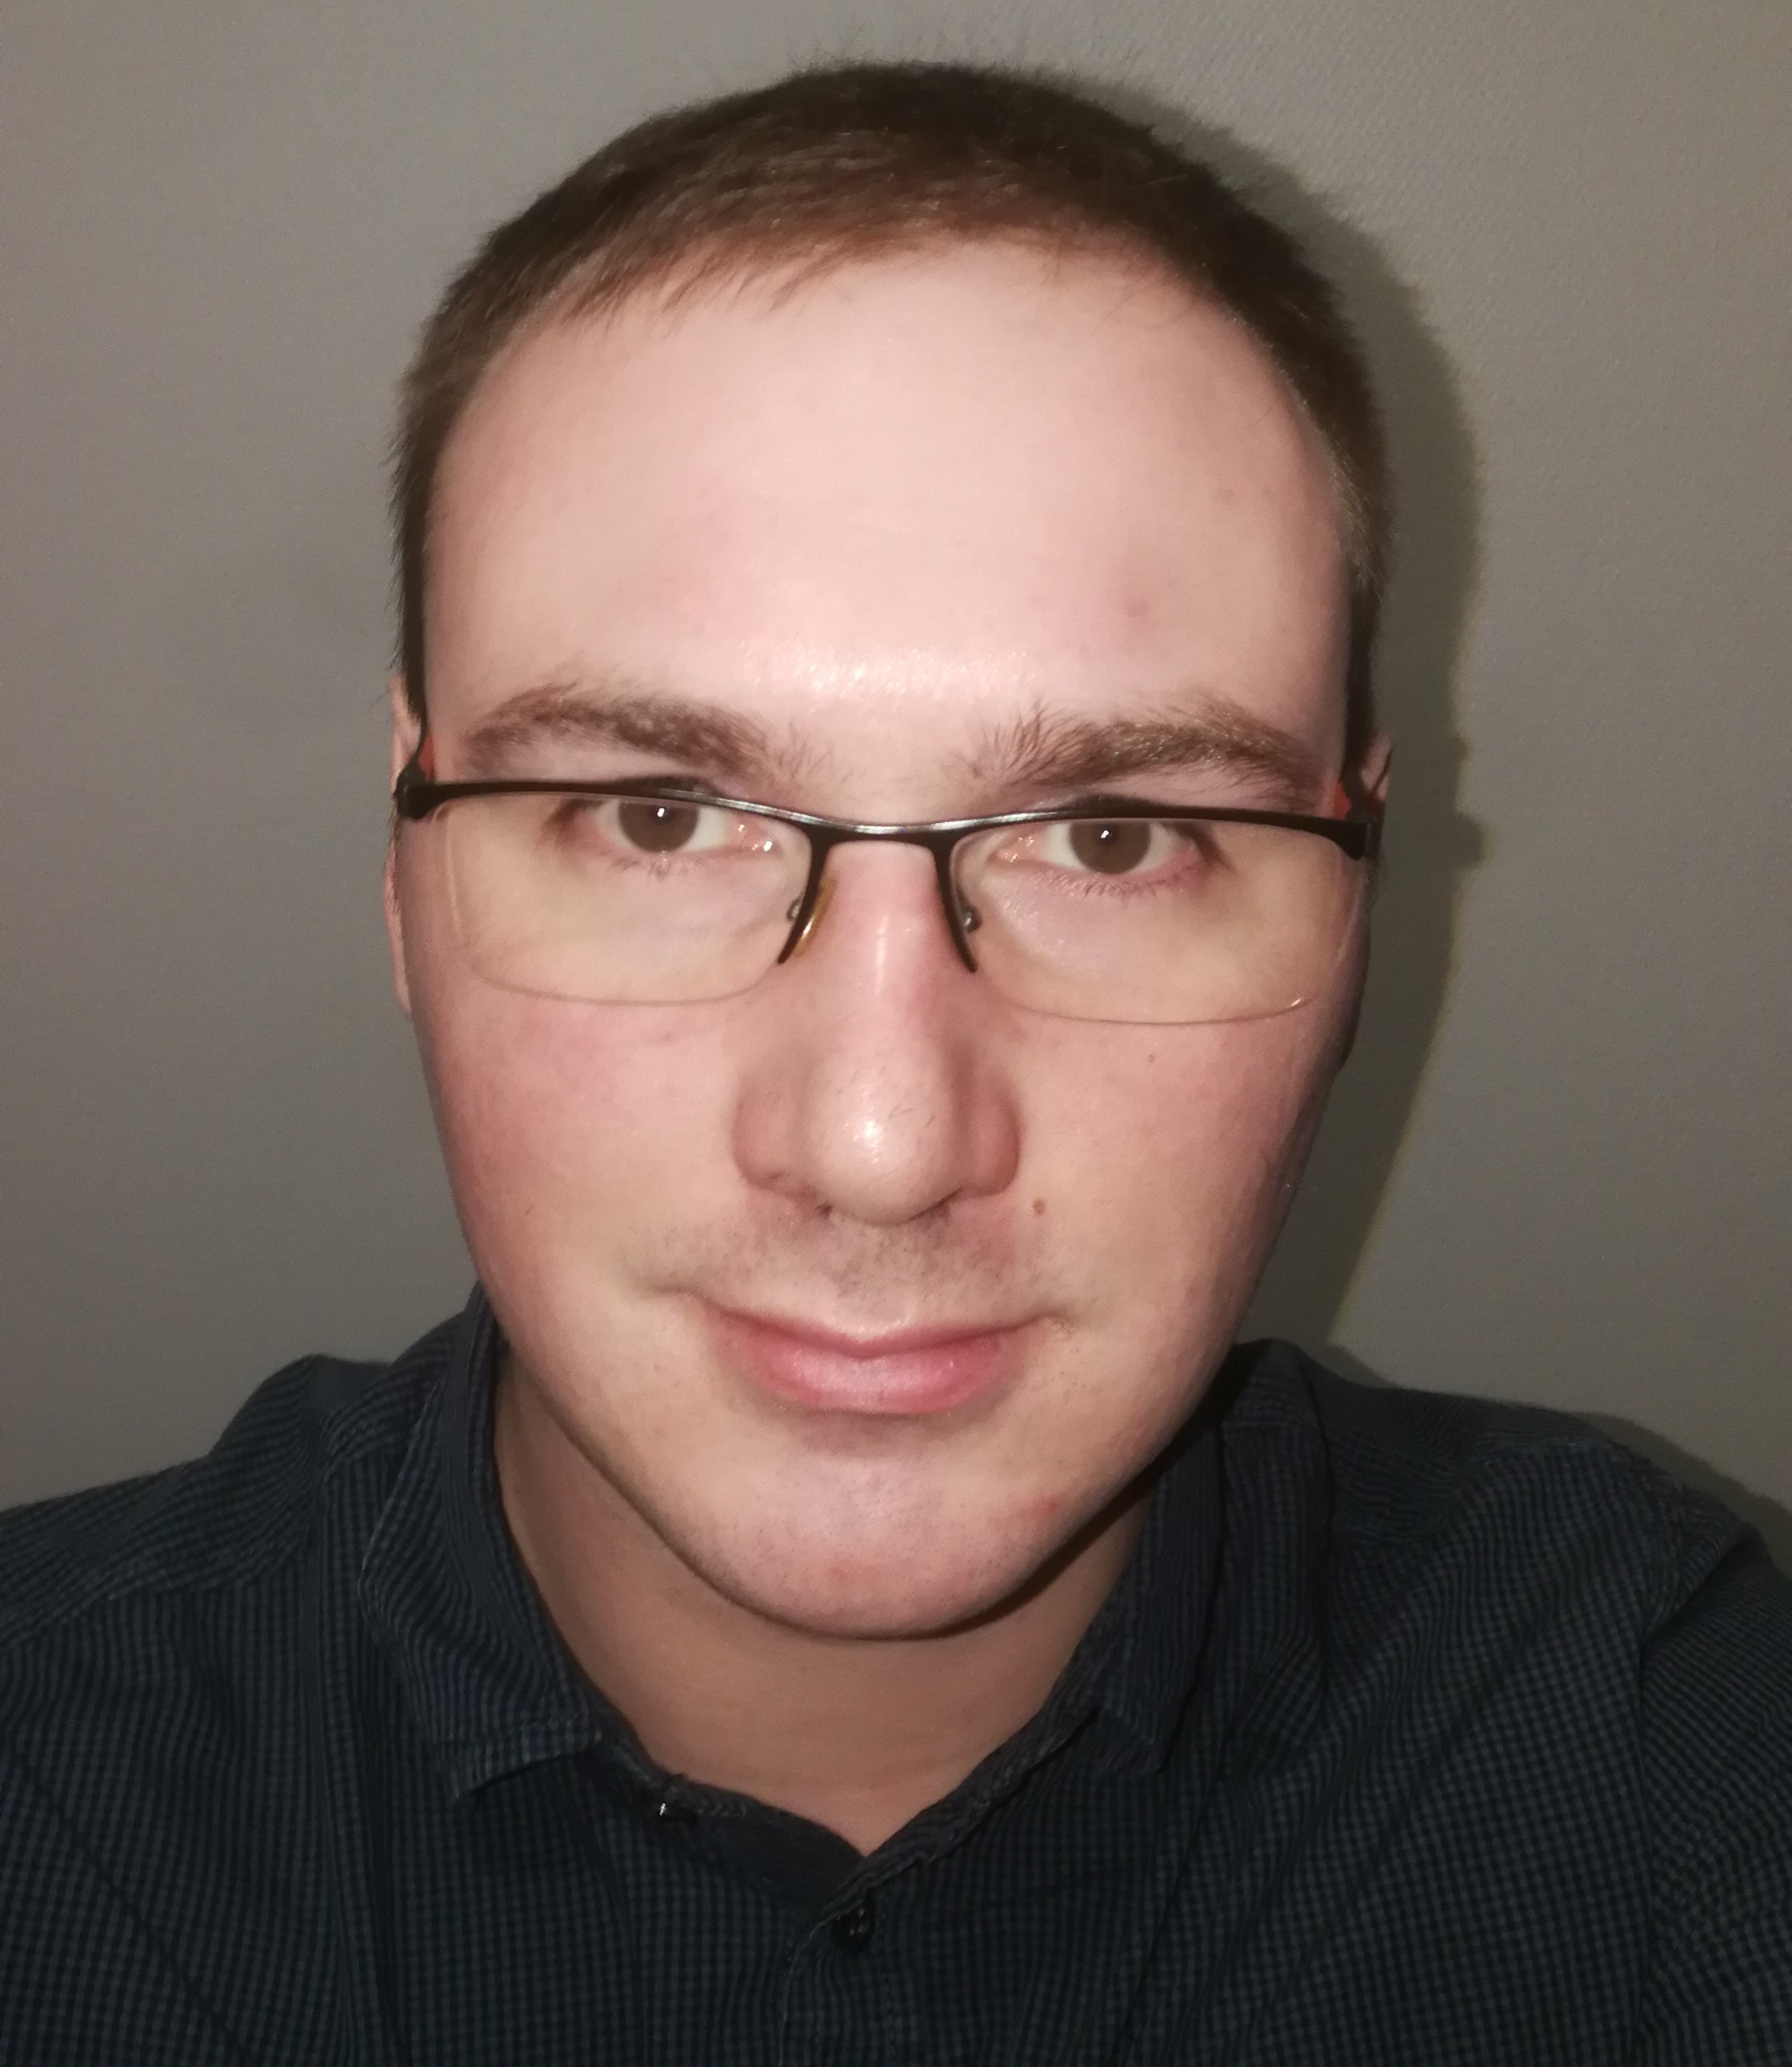
\includegraphics[scale=0.03]{
		{./Images/Portrait2.jpg}
	}
}
% Paramaters
%% fancyhdr
\pagestyle{fancy} %%% Set page style to fancy
\fancyhf{} %%% Clear header and footers
\renewcommand{\headrulewidth}{0pt} %%% Remove header line
\renewcommand{\familydefault}{\sfdefault} %% Set selected font as default
%% Hyperlink
\hypersetup{
	colorlinks=true,
	linkcolor=blue,
	filecolor=blue,      
	urlcolor=blue,
	pdftitle={\firstname \familyname - \jobtitle},
	pdfauthor={\firstname \familyname}
}
%% Text, page and text background colors
\pagecolor{white}
\color{black}
\definecolor{shadecolor}{RGB}{180,180,180} %%%% Grey
\pagenumbering{gobble} %% Disable page number
% Title definition
\renewcommand\maketitle{
	\par\noindent\begin{tabular}{ c c | c c }
		\makegapedcells
		\makecell[l]{
			\portrait
		} &
		\makecell[l]{
			\huge\firstname \\
			\huge\familyname
		} &
		\makecell[l]{
			\faPhone\ \phoneNumber \\ 
			\faEnvelope\ \href{mailto:\email}{\underline{\email}} \\
			\faBirthdayCake\ \birthday
		} &
		\makecell[l]{
			\faHome\ \street \\ \hspace{1.09em} \city \\
			\faLinkedinIn\ \href{https://www.\linkedin}{\firstname \: \familyname}
		}
	\end{tabular}
	\par\hrule
	\vspace{0.2cm}
	\centering\Large \textbf{\underline{{\Large\jobtitle} application}}
}
% Body
\begin{document}
	%% Generate title
	\maketitle
	\small
	%% Professional Experience
	\vspace{-1.2cm}
	\section*{\raggedright\large\textsc{\begin{snugshade*}Experience\end{snugshade*}}}
	\vspace{-0.5cm}
	\begin{description}
		\item \textbf{May 2024 - Oct 2024 | Data Consultant} at \textbf{Keyrus}
		\begin{itemize}[noitemsep]
			\item Data engineering mission to process and centralize data.
			\begin{itemize}[noitemsep]
				\item Gather business needs and write technical specifications.
				\item Prepare, process and insert data through Snowflake SQL procedures.
				\item Implement size and functional tests. 
				\item Manage versions, monitor tickets and AGILE methodology. 
			\end{itemize}
		\end{itemize}
		\hrule
		\item \textbf{Sep 2022 - May 2024 | Developer} at \textbf{Armatis Business Consulting}
		\begin{itemize}[noitemsep]
			\item Modeling, analyzing and querying PostgreSQL databases.
			\item Automatic data processing and insertion with Talend (ETL/ELT).
			\item Calculate key performance indicators and create reports with Power BI.
		\end{itemize} 
		\hrule
		\item \textbf{Oct 2021 - Oct 2022 | Internship} at \textbf{Armatis Business Consulting}
		\begin{itemize}[noitemsep]
			\item Training to develop with Power BI.
			\item Prototyping reports and dashboards.
		\end{itemize} 
	\end{description}
	%% Skills
	\vspace{-1.5cm}
	\section*{\raggedright \large \textsc{\begin{snugshade*}Primary skills\end{snugshade*}}}
	\vspace{-0.5cm}
	\begin{description}
		\item \textbf{Analysing and processing structured and semi-structured data}
		\par\begin{tabular}{l l l}
			• SQL and PL/SQL & • Snowflake & • PostgreSQL \\
			• Talend & • Data Analysis Expression (DAX) & • Excel / VisualBasic (VBA)
		\end{tabular}
		\hrule
		\item \textbf{Data visualization}
		\par\begin{tabular}{l l l}
			• Microsoft Power BI & • Tableau & • SAP BO Business Intelligence
		\end{tabular}
		\hrule
		\item \textbf{Relational databases modeling}
		\par\begin{tabular}{l l l}
			• UML & • Entity / Association model & • Merise methodology
		\end{tabular}
		\hrule
		\item \textbf{Cooperative software development}
		\par\begin{tabular}{l l l l}
			• GitHub / GitLab & • Confluence & • Jira & • AGILE methodology
		\end{tabular}
	\end{description}
	%% Soft skills
	\vspace{-1.5cm}
	\section*{\raggedright \large \begin{snugshade*}\textsc{Secondary skills}\end{snugshade*}}
	\vspace{-0.5cm}
	\begin{description}
		\item \textbf{French}
		\par Native speaker.
		\hrule
		\item \textbf{English}
		\par Fluent, C1 level (TOEIC certification 2022). 
		\hrule
		\item \textbf{Programming}
		\par\begin{tabular}{l l l l}
			• Python & • Java & • Unit tests & • {\normalsize\fontfamily{cmr}\selectfont \LaTeX}
		\end{tabular}
	\end{description}
	%% Studies
	\vspace{-1.5cm}
	\section*{\raggedright \large \begin{snugshade*}\textsc{Studies}\end{snugshade*}}
	\vspace{-0.5cm}
	\begin{description}
		\item \textbf{2021 - 2022 | Bachelor's degree of Big Data Developer (LP BDB)} 
		\par\hspace{1.45cm} University of Bordeaux at Périgeux's IUT
		\item \textbf{2018 - 2020 | Bachelor's degree of Statistics and Business Intelligence (DUT STID)\,} 
		\par\hspace{1.45cm} University of Poitiers at Niort's IUT
		\item \textbf{2015 - 2017 | Game Design Bachelor} 
		\par\hspace{1.45cm} Bellecour School at Lyon
		\item \textbf{2013 - 2014 | First year coursework of Management and Communication}
		\par\hspace{1.45cm} Institute of Communication Strategies and Techniques (ISTC) at Lille
		\item \textbf{2012 - 2013 | First year coursework of Economy and Management License} 
		\par\hspace{1.45cm} Private Catholic University of Economics and Management (FLSEG) at Lille
	\end{description}
	\fancyfoot[C]{\faGithub \href{https://www.\gitHubLink}{ \, \underline{GitHub}}}
\end{document}

